\documentclass[12pt, a4paper]{article}
\usepackage[utf8]{inputenc} 
\usepackage[margin=1.2in]{geometry}

\usepackage{multicol}
\usepackage{multirow}
\usepackage{url}
\usepackage{graphicx}
\usepackage{tikz}
\usepackage{xcolor}
\usepackage[utf8]{inputenc}
\usepackage{minted}
\usepackage{amsmath}
\usepackage{bm}

\title{
	\line(1,0){300}
	\endgraf\bigskip
	\Huge
	\begin{center}
		\emph{\Large{\textbf{Dijkstra's Algorithm}}}
	\end{center}
	\line(1,0){300}
	\bigskip
	\bigskip
}

\author{
	\textbf{Md. Irtiaz Kabir}\\Student ID: 2005070\\\\
	\textbf{Sadatul Islam Sadi}\\Student ID: 2005077\\\\
        \textbf{Wahid Al Azad Navid}\\Student ID: 2005089\\\\\\\\
	Department of Computer Science and Engineering\\
    Bangladesh University of Engineering and Technology\\
}

\date{
	\endgraf\bigskip
	{\today}
}

\begin{document}
    \maketitle
    \pagebreak
    \tableofcontents
    \pagebreak
    \listoffigures
    \pagebreak
    \listoftables
    \pagebreak
    \section{Introduction}
    This report briefly describes Dijkstra's algorithm for solving the single source shortest path problem. From a single source, this algorithm determines the shortest path to every node.
    \subsection{Problem Definition}
    Given a directed or undirected weighted graph with $n$ vertices and $m$ edges. The weights of all edges are non-negative. You are also given a starting vertex $s$. Under single source shortest path problem we have to find the lengths of the shortest paths from a starting vertex $s$ to all other vertices, and output the shortest paths themselves. The pure brute force solution to this problem is not feasible. One of the earliest algorithms to solve the SSSP problem in polynomial time was Dijkstra's.
    \subsection{Definition}
    Dijkstra’s algorithm is the iterative algorithmic process to provide us with the shortest path from one specific starting node to all other nodes of a graph. It applies the greedy algorithm as the basis principle. This algorithm takes a graph and a source as an input and outputs the shortest path to all other nodes in linear space complexity.
    \\\\
    \begin{figure}[h]
        \centering
        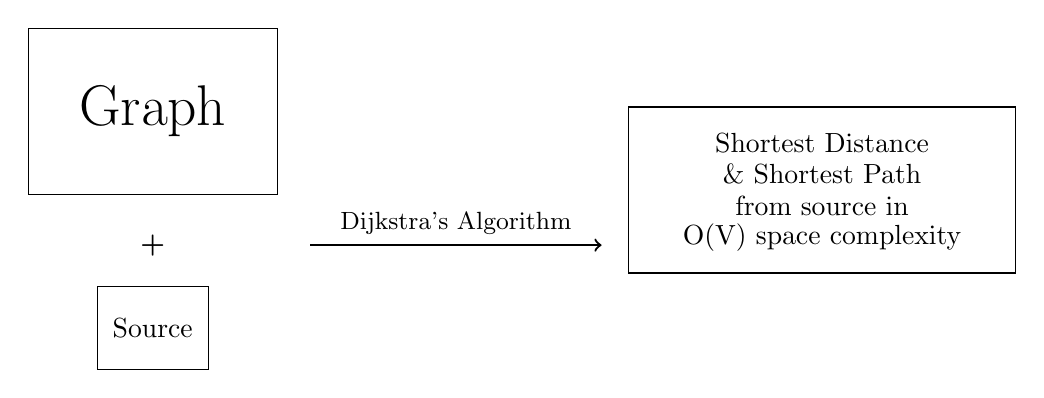
\begin{tikzpicture}
            \node[draw=black, rectangle, minimum width=90pt, minimum height=60pt](rect) at (-4,3){\textcolor{black}{\huge Graph}};
            \node[black] at (-4,1.3) {\textbf{+}};
            \node[draw=black, rectangle, minimum width=40pt, minimum height=30pt](source) at (-4,0.25){\textcolor{black}{Source}};
                % \onslide<3->
            \node[draw=black, rectangle, minimum width=140pt, minimum height=60pt](rect2) at (4.5,2){};
            \node[rectangle, black, minimum width=70pt, minimum height=40pt](text1) at (4.5,2.6){ Shortest Distance};
            \node[rectangle, black, minimum width=70pt, minimum height=40pt](text2) at (4.5,2.2){ \& Shortest Path};
            \node[rectangle, black, minimum width=70pt, minimum height=40pt](text3) at (4.5,1.8){ from source in };
            \node[rectangle, black, minimum width=70pt, minimum height=40pt](text4) at (4.5,1.4){ O(V) space complexity };
            \draw[->, thick, black] (-2,1.3) -- (1.7,1.3) node[midway, above] {\small Dijkstra's Algorithm};
        \end{tikzpicture}
        \caption{Basic input and output of Dijkstra's Algorithm}
    \end{figure}
    \pagebreak
    \section{Dijkstra's Algorithm}
    \subsection{Algorithm}
    \begin{description}
        \item[\textbf{Step 1: }] Create a priority queue\footnote{A priority queue is a type of queue that arranges elements based on their priority values. Elements with higher priority values are typically retrieved before elements with lower priority values.}, $Q$. Also define two arrays \textit{dist} and \textit{prev}
        \begin{description}
            \item[\textbf{dist: }] This array contains shortest distance so far to each node.
            \item[\textbf{prev: }] This array contains the predecessor of the node. $prev[u]$ refers to the node that has set the shortest distance of $u$.
        \end{description}
        \item[\textbf{Step 2: }]  Initially $dist[s] = 0$, and for all other vertices this length equals $\infty$. For all nodes $v \in G.V$, $prev[v] = None$.
        \item[\textbf{Step 3: }] The Dijkstra's algorithm runs for $n$ iterations. At each iteration a vertex $v$ is chosen as unvisited vertex which has the least value. We use extracMin of the priority queue for this purpose.
        \item[\textbf{Step 4: }] Next, from vertex $v$ relaxations \footnote{The Edge Relaxation property is defined as the operation of relaxing an edge u → v by checking whether the best-known way from S(source) to v is to go from S → v or by going through the edge u → v. If it is the latter case we update the path to this minimum cost.} are performed: all edges of the form $(v,\text{to})$ are considered, and for each vertex $\text{to}$ the algorithm tries to improve the value $dist[\text{to}]$. If the length of the current edge equals $len$, the code for relaxation is:
        $$dist[\text{to}] = min(dist[\text{to}], dist[v]+len)$$
        To get the actual path we use an array of predecessaors. Building this array of predecessors is very simple: for each successful relaxation, i.e. when for some selected vertex $v$, there is an improvement in the distance to some vertex $\text{to}$, we update the predecessor vertex for $\text{to}$ with vertex $v$:
        $$prev[\text{to}] = v$$
        Also we need to perform a decrease key for vertex $to$ whenever we perform a relaxation. After all such edges are considered, the current iteration ends. Finally, after $n$ iterations, all vertices will be marked, and the algorithm terminates.
        \item[\textbf{Step 5: }] Now, dist[u] shows the shortest distance from source to u. From the predecessor array of prev we can easily get the shortest path: starting with $v$, repeatedly take the predecessor of the current vertex until we reach the starting vertex $s$ to get the required shortest path with vertices listed in reverse order. So, the shortest path $P$ to the vertex $v$ is equal to: 
        $$P = (s,...,p[p[p[v]]], p[p[v]], p[v], v)$$
    \end{description}
    \pagebreak
    \subsection{Pseudo Code}
    \begin{minted}[escapeinside=||, xleftmargin=20pt,fontsize={\fontsize{12}{12}\selectfont}, linenos]{python}
        def Dijkstra(Graph, source):

        Q |$\leftarrow$| PrioriyQueue()
        dist |$\leftarrow$| |$\phi$|
        prev |$\leftarrow$| |$\phi$|

        for each vertex v in Graph.Vertices:
            dist[v] |$\leftarrow$| |$\infty$| if v is not source else 0
            prev[v] |$\leftarrow$| None
            Q.enqueue(v, dist[v])

        while Q is not empty:
            u |$\leftarrow$| Q.extract_min()

            for each neighbor v of u:
                alt |$\leftarrow$| dist[u] + Graph.Edges(u, v)
            
                if alt < dist[v]:
                    dist[v] |$\leftarrow$| alt
                    prev[v] |$\leftarrow$| u
                    Q.decrease_priority(v, alt)
                
        return dist, prev
    \end{minted}
    \pagebreak
    \section{Analysis}
\subsection{Proof of Correctness}

Let's call our source vertex $s$. Let $d(v)$ be the distance assigned by the algorithm and let $\delta(v)$ be the shortest path distance from $s$-to-$v$. We want to show that at the end of the algorithm, $\forall v,\ d(v) = \delta(v)$. This suffices to prove that the algorithm correctly computes the distances. We prove this by induction on $|Q|$ via the following lemma:\\

\noindent
\textbf{Lemma:} For each $x \in R, d(x) = \delta(x)$.
\\

\noindent
\textbf{Proof by Induction:}
\textit{Base case:} Since $Q$ only grows in size, the only time $|Q| = 1$ is when $Q = {s}$ and $d(s) = 0 = \delta(s)$, which is correct.
\\

\noindent
\textit{Inductive hypothesis:} Let $u$ be the last vertex added to $Q$. Let $Q'= Q \cup \{u\}$. Our I.H. is: for each $x \in Q'$, $d(x) = \delta(x)$
\\

\noindent
\textit{Using the I.H:} By the inductive hypothesis, for every vertex in $Q'$ that isn't $u$, we have correct distance assigned. We need only show that $d(u) = \delta(u)$ to complete the proof. \\

\noindent
Suppose for a contradiction that the shortest path from $s$-to-$u$ is $P$ and has length
\begin{equation}
    l(P) < d(u)
    \label{equation:proof-1}
\end{equation}

and at some leaves $Q'$ (to get to $u$ which is not in $Q'$). Let $xy$ be the first edge along $P$ that leaves $Q'$. Let $P_x$ be the $s$-to-$x$ subpath of $P$. Clearly:
$$l(P_x) + l(xy) \leq l(P)$$
Dijkstra's algorithm only works for non negative edge weights. If $l(xy) \geq 0$ we can rewrite it to be
\begin{equation}
    l(P_x) < l(P)
    \label{equation:proof-2}
\end{equation}

Since $d(x)$ is the length of the shortest $s$-to-$x$ path by I.H., $d(x) \leq l(P_x)$, giving us
\begin{equation}
    d(x) + l(xy) \leq l(P_x)
    \label{equation:proof-3}
\end{equation}

Since $y$ is adjacent to $x$, $d(y)$ must have been updated by the algorithm, so
\begin{equation}
    d(y) \leq d(x) + l(xy)
    \label{equation:proof-4}
\end{equation}

Finally, since $u$ was picked by the algorithm, $u$ must have the smallest distance assigned -
\begin{equation}
    d(u) \leq d(y)
    \label{equation:proof-5}
\end{equation}

\noindent
Combining equation (\ref{equation:proof-1}), (\ref{equation:proof-2}), (\ref{equation:proof-3}), (\ref{equation:proof-4}), (\ref{equation:proof-5}) we get,

$$d(u) \leq d(y) \leq d(x) + l(xy) \leq l(P_x) < l(P) < d(u)$$
Which implies $d(u) < d(u)$ - a contradiction. Therefore, no such shorter path $P$ can exist and so $d(u) = \delta(u)$.\\

So the lemma holds, which proves that at the end of the algorithm, every vertex has been assigned the shortest distance from the source vertex.

\subsection{Running Time}
The algorithm takes different running time for different implementation for the abstract data structures used (graph and priority queue). But there is a fixed bottleneck for most common implementations. There are mainly 2 stages of the algorithm - 

\begin{description}
    \item[Initialization stage] Initializing the $dist$ and $prev$ arrays, enqueuing the vertices
    \item[Iteration stage] Iterating through the vertices one by one in increasing order of their priority and updating the $dist$ and $prev$ arrays and priorities of the vertices
\end{description}

\noindent
For every implementation the iteration stage becomes the bottleneck. That is because the initialization stage simply iterates through the vertices in $O(|V|)$ running time ($|V|$ denotes the number of vertices and $|E|$ denotes the number of edges). But the iteration stage is costlier. So far we haven't found an implementation that can perform the iteration stage in $O(|V|)$).
\\

\noindent
There are mainly 2 operations that make the iteration stage the bottleneck of the whole algorithm. $extract\_min$ and $decrease\_priority$. Different implementations handle these operations differently than one another. But we can generalize the overall running time in an abstract fashion.
\\
\noindent
\textbf{Analyzing the bottleneck operations:}
\begin{description}
    \item[Extract Min] This is called $\Theta(|V|)$ times because each vertex is enqueued exactly once in the initialization stage and never again
    \item[Decrease Priority] This is called for each neighbor of a vertex. This is done by traversing the edges of a vertex. And since this traversal takes place for every single vertex, all the edges are traversed eventually. So $decrease\_priority$ is called $\Theta(|E|)$ times
\end{description}
Let, for a specific implementation, the running time of $extract\_min$ is $T_{em}$ and the running time of $decrease\_priority$ is $T_{dp}$\\

\noindent
So the overall running time,
$$T = \Theta(|V|) \times T_{em} + \Theta(|E|) \times T_{dp}$$

\noindent
Different implementation have different $T_{em}$ and $T_{dp}$

\begin{table}[h]
    \centering
    \begin{tabular}{| c | c | c | c |}
        \hline
        \textbf{Implementation} & \boldsymbol{$T_{dp}$} & \boldsymbol{$T_{em}$} & \boldsymbol{$T$} \\
        \hline
        Singly Linked List & $\Theta(1)$ & $\Theta(|V|)$ & $\Theta(V^2)$\\
        Binary Min Heap & $\Theta(log|V|)$ & $\Theta(log|V|)$ & $\Theta\left((E + V)log|V|\right)$\\
        Fibonacci Heap & $\Theta(1)$ & $\Theta(log|V|)$ & $\Theta(E + Vlog|V|)$ \\
        \hline
    \end{tabular}
    \caption{Running Time for Different Implementations}
\end{table}

So far the use of a Fibonacci Heap is found to be the most optimal.
\begin{figure}[h]
    \centering
    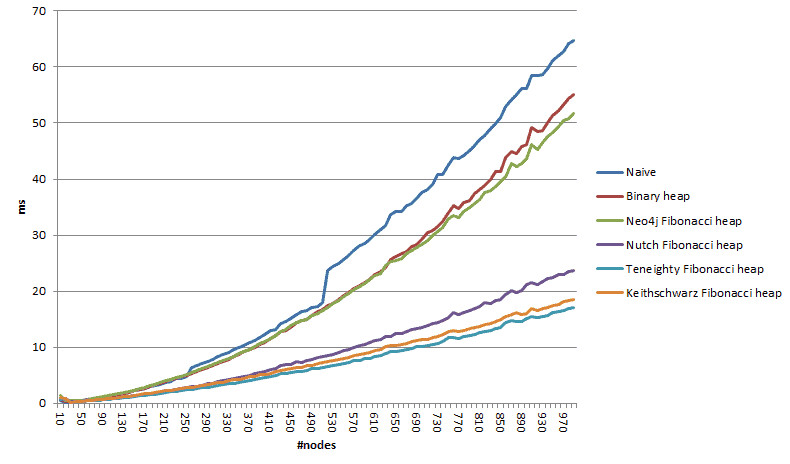
\includegraphics[width=\textwidth]{benchmark.jpg}
    \caption{Benchmarking Different Implementations}
    \cite{baeldung_2022}
\end{figure}



\clearpage

\section{Drawbacks}
\subsection{Traversing Unnecessarily}

 \textit{Dijkstra's} algorithm guarantees to produce the accurate result for both directed and undirected graphs. However, it may result in a longer running time for certain graphs.

\par For instance, in this graph, our objective is to determine the most efficient route from the starting point (\textit{S}) to the destination (\textit{D}). 

\vspace{1cm}






\begin{figure}[h]
    \centering
    
    \begin{tabular}{ccc}
        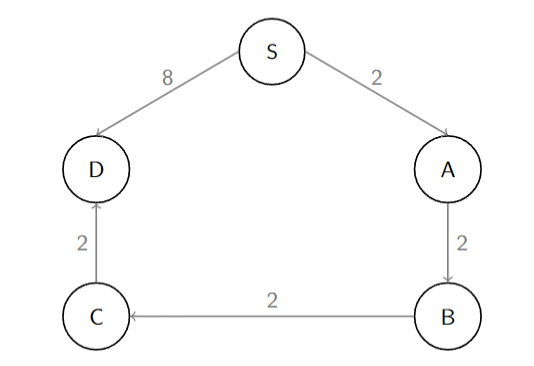
\includegraphics[width=0.33\textwidth]{Images/1.png} & 
        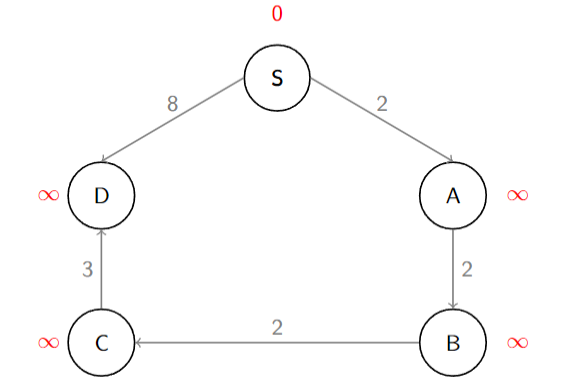
\includegraphics[width=0.33\textwidth]{Images/2.png} &
        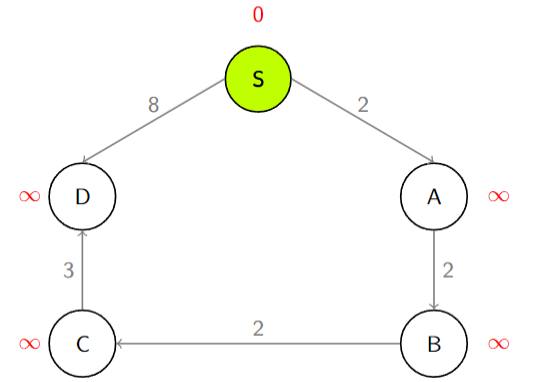
\includegraphics[width=0.33\textwidth]{Images/3.png} \\
    

        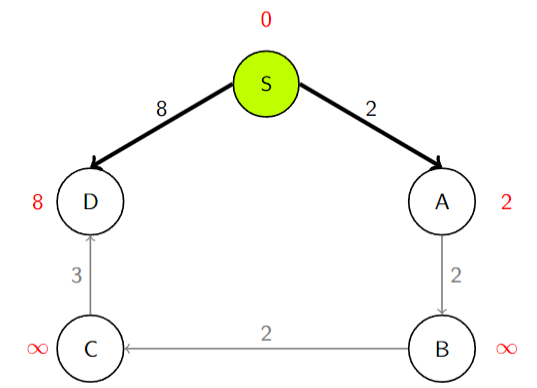
\includegraphics[width=0.33\textwidth]{Images/4.png} & 
        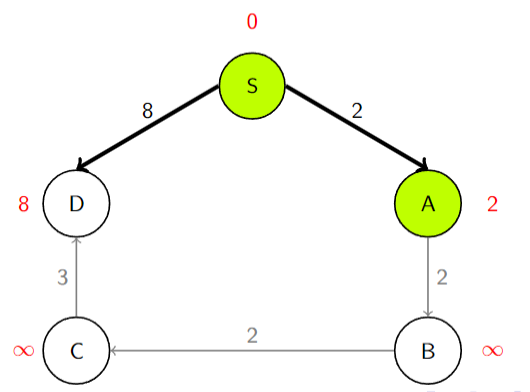
\includegraphics[width=0.33\textwidth]{Images/5.png} &
        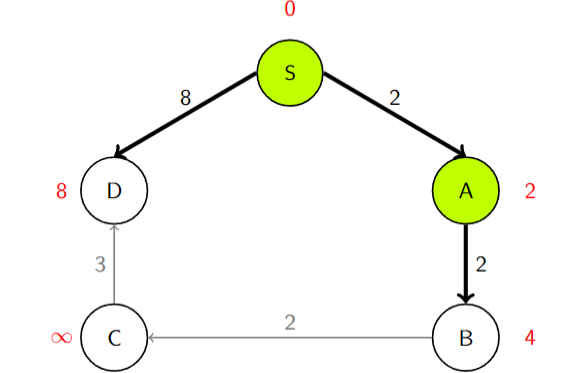
\includegraphics[width=0.33\textwidth]{Images/6.png} \\

   

        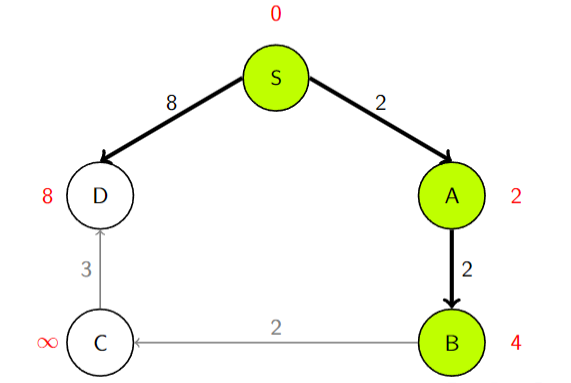
\includegraphics[width=0.33\textwidth]{Images/7.png} & 
        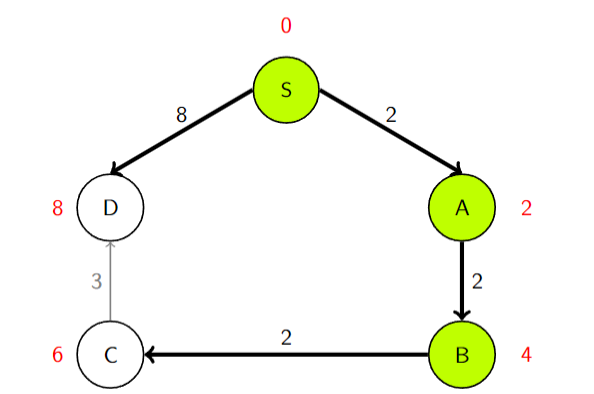
\includegraphics[width=0.33\textwidth]{Images/8.png} &
        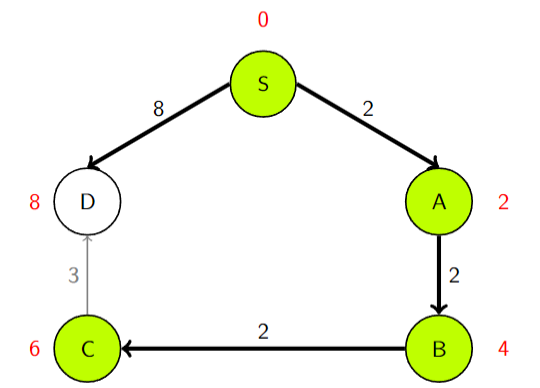
\includegraphics[width=0.33\textwidth]{Images/9.png} \\

    

        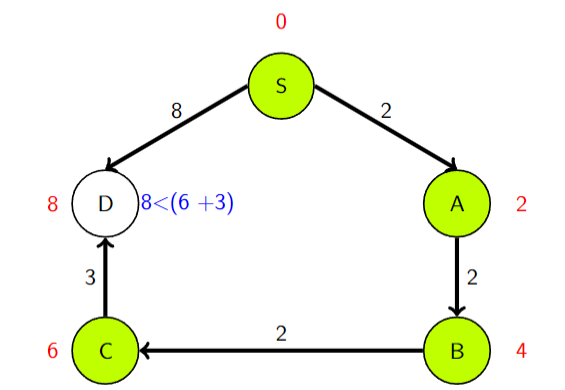
\includegraphics[width=0.33\textwidth]{Images/10.png} & 
        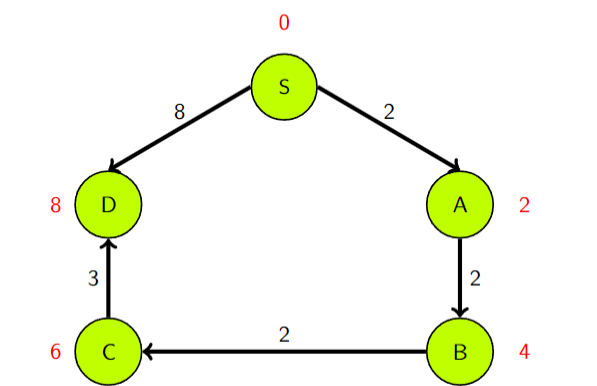
\includegraphics[width=0.33\textwidth]{Images/11.png} &
         \\
    \end{tabular}
    \caption{Extended traversal caused by \textit{Dijkstra's} Algorithm}
    \label{fig:my_label}
\end{figure}

\par Even though the points are in close adjacency to each other, implementing \textit{Dijkstra's} algorithm would necessitate traversing the entire graph to identify the shortest path.

\subsection{Inability to Handle Negative-Weight Edges}

\par The algorithm falls short in finding the shortest path between nodes or from a single node to all others. Due to its greedy nature, it selects the most favorable path available at each step. However, the presence of negative-weight edges introduces the possibility of a more optimal route utilizing edges that the algorithm may disregard during intermediate stages.


\section{Specialized Variants}
When arc weights are small integers(bounded by a parameter \textbf{\textit{C}}), specialized queues which ake advantage of this fact can be used to speed up \textit{Dijkstra's} algorithm.
\begin{itemize}
    \item The first algorithm of this type was \textbf{Dial's algorithm} \cite{dial1969algorithm} for graphs with positive integer edge weights, which uses a bucket queue to obtain a running time of {$O(|E| + |V|*C)$}.
    \item  The use of a \textbf{Van Emde Boas tree} \cite{vanvan} as the priority queue brings the complexity to {$O(|E|  * loglogC)$}.

    \item Another interesting variant based on a combination of a new radix heap and the well-known Fibonacci heap runs in time {$O(|E| + |V| \sqrt{logC})$} which was properposed by \textbf{Ahuja et. al}\textit{(1990)}  \cite{ahuja1990faster}.

    \item Finally, the best algorithm in this case was given by \textbf{Thorup}\textit{(2000)} \cite{thorup2000ram} which runs in {$O(|E|  * loglogV)$}.


\end{itemize}



\section{Applications}



\textit{Dijkstra's} algorithm is commonly used in various domains such as computer networking, transportation systems, and geographic information systems (GIS). In this section, we explore and discuss different application scenarios to illustrate how the algorithm plays a crucial role in solving practical problems within these contexts.

\subsection{Routing in Computer Networks}
\begin{itemize}
  \item \textit{Dijkstra}'s algorithm, utilized in internet routing, dynamically adapts to varying network conditions, facilitating efficient data transmission by continually recalculating optimal routes.
  \item It enables routers to prioritize paths with minimal latency, ensuring swift and reliable communication between devices connected to the network.

\end{itemize}

\subsection{Transportation and Logistics}
\begin{itemize}
  \item Logistics companies rely on \textit{Dijkstra}'s algorithm to properly plan delivery routes, optimizing the sequence of stops to minimize fuel consumption and reduce overall transportation costs.
  \item By considering real-time traffic data and delivery constraints, the algorithm aids in dynamic route adjustments, enhancing the efficiency of last-mile delivery operations.
  \item Its application in logistics contributes to timely and cost-effective transportation solutions, impacting industries ranging from e-commerce to traditional shipping services.
\end{itemize}

\subsection{Network Routing Protocols}
\begin{itemize}
  \item Open Shortest Path First (OSPF), a widely used routing protocol, employs \textit{Dijkstra}'s algorithm to compute the shortest paths between routers, promoting efficient data flow within complex network infrastructures.
  \item The algorithm's ability to adapt to changing network topologies enhances OSPF's resilience, ensuring rapid convergence and minimizing network downtime in response to link failures.

\end{itemize}

\subsection{Geographic Information Systems (GIS)}
\begin{itemize}
  \item Geographic Information Systems leverage \textit{Dijkstra}'s algorithm to analyze spatial data, providing valuable insights for urban planners by determining optimal routes for emergency evacuation in the event of natural disasters.
  \item The algorithm's consideration of varying terrain and obstacles enhances GIS applications' accuracy in predicting evacuation times and suggesting safe pathways for affected populations.
  
\end{itemize}

\subsection{Robotics and Autonomous Vehicles}
\begin{itemize}
  \item Autonomous vehicles utilize \textit{Dijkstra}'s algorithm for path planning, allowing them to navigate complex environments with real-time adjustments to avoid obstacles and reach destinations efficiently.
  \item The algorithm's incorporation into robotics enables adaptive decision-making, as vehicles dynamically calculate the optimal routes based on current conditions, enhancing safety and operational effectiveness.
 
\end{itemize}



\subsection{Telecommunication Network Design}
\begin{itemize}
  \item Telecommunication engineers employ \textit{Dijkstra}'s algorithm to plan fiber-optic cable routes efficiently, reducing signal transmission latency and optimizing the overall design of communication networks.
  \item By considering factors such as cable length and transmission speeds, the algorithm aids in designing networks that meet the demands of high-speed data transfer and communication reliability.

\end{itemize}

\subsection{Game Development}
\begin{itemize}
  \item In video game development, \textit{Dijkstra}'s algorithm ensures that non-player characters (NPCs) navigate game environments seamlessly, enhancing the overall gaming experience by providing realistic and adaptive character movements.
  \item The algorithm's integration into pathfinding algorithms allows game developers to create engaging and challenging environments where NPCs intelligently navigate obstacles and follow optimal routes.
 
\end{itemize}


\section{Conclusion}

In conclusion, Dijkstra's algorithm is a flexible and basic tool in computer science and engineering, with applications in a variety of domains. Its versatility in routing situations, resource management, and geographical analysis emphasises its importance in optimising pathways and effectively navigating complicated networks. The investigation of numerous use cases reveals that Dijkstra's algorithm plays a critical role in improving efficiency, dependability, and flexibility across a wide range of real-world systems.

As technology advances, Dijkstra's algorithm's continuous significance in routing protocols, logistics, autonomous systems, and other areas demonstrates its long-term effect. Future research and development may look at upgrades and adaptations to broaden the algorithm's capabilities and handle future difficulties in industries like telecommunications, transportation, and gaming.





\pagebreak

\bibliographystyle{abbrv}
\bibliography{ref_navid}

\end{document}